% Diapo d'intro

\begin{frame}[c]
  \frametitle{Objectifs}

La modélisation d'un système est la première étape vers sa compréhension

\begin{center}
  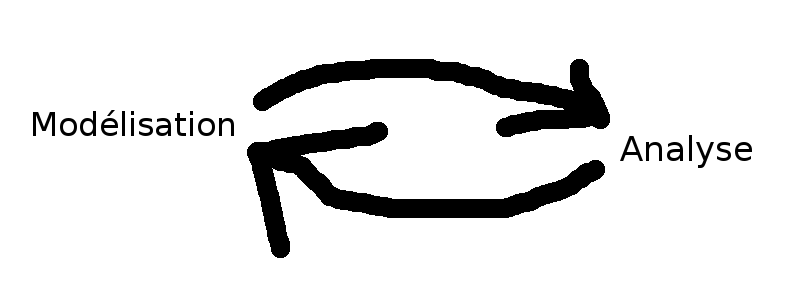
\includegraphics[width=.4\textwidth]{figs/modelanalyse.png}
\end{center}

L'analyse recherchée impacte les choix de modélisation
\begin{itemize}
  \item Les outils de modélisation doivent être adaptés aux propriétés observées
\end{itemize}

\medskip
Les choix de modélisation impactent les résultats de l'analyse
\begin{itemize}
  \item Un modèle trop grossier donne peu d'informations
  \item Un modèle de grande taille augmente le temps d'analyse
\end{itemize}

\medskip
\begin{center}
\tval{Les étapes de modélisation et d'analyse d'un système sont indissociables}
\end{center}

\end{frame}
